\section{First-principles model: details and proofs}\label{app:fp}

\paragraph{Cost model and server.} The prefill GPU time of $x$ new tokens on a cached prefix of $y$ tokens is $t_P(x,y)=a\max(1,x/B_c)+\max(f_0,bx)+c_p\,x\,(y+(x+1)/2)$, with $a=9.24$\,ms, $f_0=1.26$\,ms, $b=62.6\,\mu$s/token, $c_p=2.24$\,ns per causal pair and chunk $B_c=8192$ (\fpath{calibration/round6_server_log_fit/calibration.yaml}). For a miss, $t^m_k=t_P(L_k,0)$; for a hit, $t^h_k=t_P(551,L_k-551)$; turn~1 always misses. The mean prefill time per turn is $\bar t_P(h)=\sum_kw_kt_k(h)$, so $p=\nu\bar t_P(h)$ and $\partial_h\bar t_P=-\beta_P$. A decode iteration over $R_D$ requests takes $\tau_D(R_D)=a+\max(f_0,bR_D)+b_{\mathrm{att}}R_D$, with $b_{\mathrm{att}}=c_d\bar y_D/8192$, $c_d=0.31$\,ms and $\bar y_D$ the mean decode context. We assume: (S1) a turn's prefill latency is its own prefill GPU time, with no queueing behind other prefills; (S2) the GPU is busy whenever a request runs; (S3) a running request reserves $E_k$ from admission to completion, with no retraction. For vLLM, prefill and decode share iterations: $S_D=(d-1)/r_{\mathrm{it}}$, with iteration rate $r_{\mathrm{it}}=(1-\nu c_{\mathrm{turn}})/a$, where $c_{\mathrm{turn}}=b\bar x+c_p\bar\pi+(b+b_{\mathrm{att}})(d-1)$ is the token-proportional GPU time of a turn ($\bar x$ and $\bar\pi$ are the mean prefilled tokens and causal pairs per turn), as long as an iteration's tokens fit its chunk budget. Lemmas~\ref{lem:server} and~\ref{lem:rho}, and the results that use them, Proposition~\ref{prop:nb}(a) and (c), Proposition~\ref{prop:scaling}(b)--(c) and Proposition~\ref{prop:fold}, are for the separate-iteration (SGLang) server; for vLLM, $n_b$ follows from the identity of Proposition~\ref{prop:nb}(b) whenever the mixed server's $\nu_b$ exists, that is, while the chunk budget does not bind.

\begin{lemma}[fluid server]\label{lem:server}
Fix $h$, and let $\nu_{\mathrm{cap}}(h)=1/(\bar t_P(h)+(d-1)(b+b_{\mathrm{att}}))$. For $\nu<\nu_{\mathrm{cap}}(h)$ the decode equation has exactly one positive root; for $\nu\ge\nu_{\mathrm{cap}}(h)$ it has none. $S_D$ is continuous, strictly increasing in $\nu$, non-increasing in $h$, and $S_D\to\infty$ as $\nu\uparrow\nu_{\mathrm{cap}}(h)$. $K_{\mathrm{run}}(\nu,h)$ increases strictly in $\nu$ from $0$ to $\infty$ and decreases strictly in $h$.
\end{lemma}
\begin{proof}
$\psi(R)=R/\tau_D(R)$ is continuous and strictly increasing, since $\tau_D$ is affine with positive intercept on each side of the kink $f_0/b$. Moreover $\psi(0)=0$ and $\psi(\infty)=1/(b+b_{\mathrm{att}})$. The decode equation reads $\psi(R_D)=\nu(d-1)/(1-p)$, which has a unique root if and only if the right side is below $1/(b+b_{\mathrm{att}})$, that is, $\nu<\nu_{\mathrm{cap}}(h)$. The right side increases in $\nu$ and does not increase in $h$, because $t^h_k\le t^m_k$; so does $R_D$, which diverges at $\nu_{\mathrm{cap}}$. Then $S_D=R_D/\nu=(d-1)\tau_D(R_D)/(1-p)$ is a product of positive factors with the same monotonicity. $K_{\mathrm{run}}=\nu\sum_kw_kE_k(t_k(h)+S_D)$ inherits it; strict decrease in $h$ follows from $\partial_hK_{\mathrm{run}}=-\nu(\beta_E+\bar E\chi\xi)<0$ (Lemma~\ref{lem:rho}).
\end{proof}

\begin{lemma}[decode sensitivity]\label{lem:rho}
Away from the kink, $-\partial_hS_D=\chi\,\nu\partial_\nu S_D$, with $\chi=\beta_P/(\bar t_P(h)+(d-1)\tau_D'(R_D))$ and $\nu\partial_\nu S_D=R_D(\bar t_P+(d-1)\tau_D')/J>0$, where $J=(1-p)-\nu(d-1)\tau_D'>0$.
\end{lemma}
\begin{proof}
Write $G(R_D,\nu,h)=R_D(1-\nu\bar t_P(h))-\nu(d-1)\tau_D(R_D)$. Then $\partial_{R_D}G=J$; at the root, $J=(1-p)\alpha_D/\tau_D>0$, with $\alpha_D>0$ the intercept of the affine piece of $\tau_D$. Next, $\partial_\nu G=-R_D\bar t_P-(d-1)\tau_D$ and $\partial_hG=\nu R_D\beta_P$, since $\partial_h\bar t_P=-\beta_P$. Hence $\partial_hS_D=\partial_hR_D/\nu=-R_D\beta_P/J$ and $\nu\partial_\nu S_D=\partial_\nu R_D-R_D/\nu=[R_D\bar t_P+(d-1)\tau_D-JR_D/\nu]/J$. Substituting $JR_D/\nu=R_D/\nu-R_D\bar t_P-R_D(d-1)\tau_D'$ and $R_D/\nu=(d-1)\tau_D/(1-p)$ gives $(d-1)\tau_D-R_D/\nu=-pR_D/\nu=-\bar t_PR_D$, so the numerator equals $R_D(\bar t_P+(d-1)\tau_D')$.
\end{proof}

\begin{proof}[Proof of Proposition~\ref{prop:nb}]
(a) Fix $R>0$ and $h=F_Z(R)$. The function $\nu\mapsto K_{\mathrm{run}}(\nu,h)+\nu\mathcal D(R)/E[T]-M$ is continuous and strictly increasing (Lemma~\ref{lem:server}). It equals $-M$ at $\nu=0$ and is unbounded at $\nu_{\mathrm{cap}}$, so it has exactly one root $\nu(R)$, which is continuous in $R$. A state with a queue has $K_{\mathrm{run}}=M$, so $\mu\mathcal D=0$, hence $R=0$, $h=0$ and $\nu=\nu_b$. From $\nu\mathcal D(R)/E[T]\le M$ and $\mathcal D(R)\ge E[E_T]R$ we get $\nu(R)\to0$ as $R\to\infty$. As $R\downarrow0$, $\nu(R)\to\nu_b$ by continuity, since $\nu_{\mathrm{cap}}(0)$ is excluded. So $n(R)$ is bounded on $(0,\infty)$, and beyond its supremum and $n_b$ only the all-miss state remains.
(b) $K_{\mathrm{run}}(\nu_b,0)=\nu_b\sum_kw_kE_kS_k=M$ gives $\nu_b\bar S=M/E_S$; Little's law with no queue gives $n_b=\nu_b\bar S+\nu_b\bar z'$. For $n>n_b$ the all-miss state carries a queue of $(n-n_b)/\nu_b$ seconds.
(c) Divide every cost by $s$ and time by $s$: every service time scales by $1/s$ and every rate by $s$, and the decode equation and $p$ are invariant. So $(\nu,h)$ solves $K_{\mathrm{run}}=M$ for costs $\mathcal C$ if and only if $(s\nu,h)$ does for $\mathcal C/s$. Hence $\nu_b(s)=s\nu_b(1)$; $E_S$, a ratio of $S$-weighted sums, is invariant; substitute into (b).
\end{proof}

\begin{proof}[Proof of Proposition~\ref{prop:scaling}]
(a) Rescaling time by $s$ maps a stationary state $(n,\nu,h,R)$ of $(\mathcal C/s,\bar z)$ to $(n,\nu/s,h,sR)$ of $(\mathcal C,s\bar z)$. Each equation of Eq.~\eqref{eq:balance} is invariant: Little's law and $K_{\mathrm{run}}$ are rate$\times$time, $E[\min(\bar zY,R)]=s^{-1}E[\min(s\bar zY,sR)]$, and $h$ compares times. Both $\mu^*$ and $\mu_b$ scale by $s$, so their ratio depends on $s\bar z$ only.
(b) Parametrize the queue-free states by $h\in(0,1)$, with $r(h)=F_Y^{-1}(h)$ and $m(h)=E[\min(Y,r(h))]$. The balance reads $K_{\mathrm{run}}(\nu,h)+\nu\bar z(A_1m(h)+E[E_T]r(h))/E[T]=M$. Its left side increases strictly in $\nu$ and in $\bar z$, so $\nu(h;\bar z)$ decreases strictly in $\bar z$, while $\nu_b$ (the equation at $h=0$) does not involve $\bar z$. Taking the supremum over $h$, $\omega$ is non-increasing in $\bar z$. For strictness, let $\bar z_1<\bar z_2$ and $\omega>1$ at $\bar z_2$. Then $\sup_h\nu(h;\bar z_2)>\nu_b$; since $\nu(\cdot;\bar z_2)$ is continuous, tends to $\nu_b$ as $h\to0$ and to 0 as $h\to1$ (where $r(h)\to\infty$), the supremum is attained at some $h_2\in(0,1)$, and $\sup_h\nu(h;\bar z_2)=\nu(h_2;\bar z_2)<\nu(h_2;\bar z_1)\le\sup_h\nu(h;\bar z_1)$. Apply (a) for $s$.
(c) For $h\ge h_0>0$, $\nu(h;\bar z)\le ME[T]/(\bar z(A_1m(h_0)+E[E_T]r(h_0)))\to0$. For $h<h_0$, $\nu(h;\bar z)$ is below the root of $K_{\mathrm{run}}(\nu,h)=M$, which tends to $\nu_b$ as $h_0\to0$.
\end{proof}

\begin{proof}[Proof sketch of Proposition~\ref{prop:fold}]
We work away from the $R$ at which $R_D$ crosses the kink of $\tau_D$, where Lemma~\ref{lem:rho} applies; at that $R$ the same computation holds with one-sided derivatives. On the branch, $\Gamma(\nu,R)=\nu S_E(\nu,h)+\nu\mathcal D(R)/E[T]-M=0$ and $n=\nu(\bar S+\bar z')$, with $h=F_Z(R)$ and $dh/dR=f(R)$. From $S_k=t_k(h)+S_D(\nu,h)$ we have $\partial_h\bar S=-\beta_P+\partial_hS_D$, $\partial_hS_E=-\beta_E+\bar E\partial_hS_D$, $\partial_\nu\bar S=\partial_\nu S_D$ and $\partial_\nu S_E=\bar E\partial_\nu S_D$. By Lemma~\ref{lem:rho}, $\partial_hS_D=-\chi\xi$ with $\xi=\nu\partial_\nu S_D$. Then $\Gamma_\nu=\partial_\nu\Gamma=S_E+\bar E\xi+\mathcal D/E[T]>0$ and $\partial_R\Gamma=-\nu f(\beta_E+\bar E\chi\xi)+\nu\mathcal D'/E[T]$, so
\[\frac{d\nu}{dR}=\frac{\nu}{\Gamma_\nu}\Big[f(\beta_E+\bar E\chi\xi)-\frac{\mathcal D'}{E[T]}\Big].\]
Next, $dn/dR=n_\nu\,d\nu/dR+\nu f\,\partial_h\bar S=n_\nu\,d\nu/dR-\nu f(\beta_P+\chi\xi)$, with $n_\nu=\bar S+\bar z'+\xi$. Put both over $\Gamma_\nu$: the coefficient of $\nu f/\Gamma_\nu$ is $I=n_\nu(\beta_E+\bar E\chi\xi)-(\beta_P+\chi\xi)\Gamma_\nu$. Expanding, the terms $\bar E\chi\xi^2$ cancel. Collecting the terms linear in $\xi$ gives $\xi[\beta_E-\bar E\beta_P+\chi(\bar E(\bar S+\bar z')-S_E-\mathcal D/E[T])]$, and the remainder is $\beta_E(\bar S+\bar z')-\beta_P(S_E+\mathcal D/E[T])$. This is the stated $I$. The term in $\mathcal D'$ is $-n_\nu\mathcal D'/E[T]$.
(a) As $R\to0^+$, $n(R)\to n_b$ (Proposition~\ref{prop:nb}), $\mathcal D\to0$ and $\mathcal D'(0^+)=A_1+E[E_T]=E[T]\bar E$. If the bracket is positive at $0^+$, then by continuity $n$ increases on some $(0,\delta)$. Since $n(R)\to0$ as $R\to\infty$, $n$ attains a maximum $n_{\mathrm{fold}}>n_b$, and by the intermediate value theorem every $n\in(n_b,n_{\mathrm{fold}})$ is reached on both sides of the maximizer. Together with the all-miss state this gives at least three stationary states. For $n>n_b$, Little's law at $h=0$ with no queue forces $\nu>\nu_b$, so $K_{\mathrm{run}}>M$; by continuity the feedback map is memory-gated ($\Phi_n\equiv0$) near $h=0$, and the all-miss state is locally stable under the relaxation defined before Proposition~\ref{prop:fold}.
(b) A strictly decreasing continuous $n(R)$ is a bijection onto $(0,n_b)$.
\emph{Window opening.} At $R\to0^+$ the formula for $d\nu/dR$ has the sign of $f(0^+)\Delta_S-1$, with $\Delta_S=(\beta_E+\bar E\chi\xi)/\bar E$. If it is positive, $\mu=\nu/E[T]$ rises above $\mu_b$ as $R$ leaves 0.
\end{proof}
\noindent This argument is a proof sketch: the algebra of the identity is given in full, but the local stability of the all-miss state rests on a continuity step that we have not written out, and the stability of the queue-free states is argued, not proved (below). The identity is also checked in magnitude: its closed form agrees with central finite differences of $n(R)$ within a relative tolerance of $2\times10^{-3}$ at five values of $R$, for the exponential law and for a folding mixture (\fpath{tests/test_theory_paper.py}). That the registered cells are fold-free is a numerical statement: the ratio $fI/(n_\nu\mathcal D'/E[T])$ was evaluated on 400 values of $R$ per cell, with complete sign agreement against finite differences of $n$ (\fpath{analysis/theory/merged/fold.py}). The stability of the queue-free states is a further statement: under relaxation $\dot h=\eta(\Phi_n(h)-h)$, $\eta>0$, and the condition $\partial_n\Phi_n<0$, which we have checked only numerically and outside the committed code, a queue-free state is stable if and only if $dn/dR<0$ there, because along the curve $n'(R)=f(R)(1-\partial_h\Phi_n)/\partial_n\Phi_n$.

\begin{figure*}[t]\centering
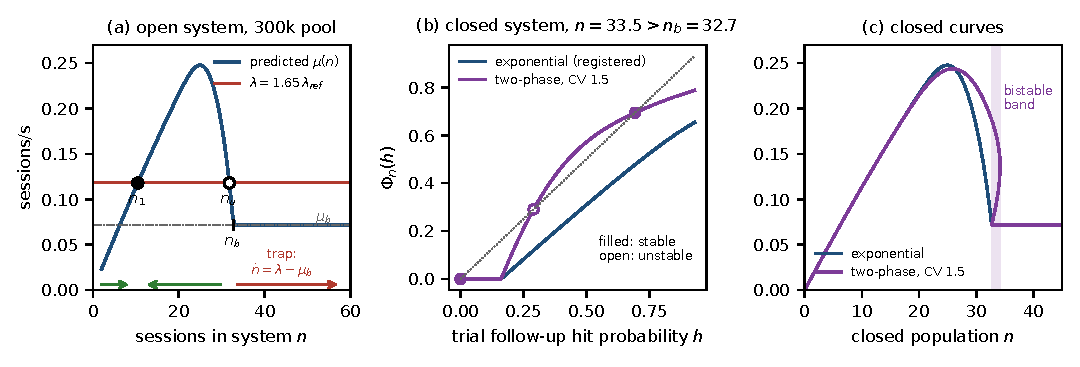
\includegraphics[width=\textwidth]{figs/fig10_theory_fixed_points.pdf}
\caption{Fixed points of the first-principles model. (a) Open system, predicted 300k curve at 1.65 $\lref$: stable good state $n_1=10.4$, unstable state $n_2=31.8$ (marked $n_u$), all-miss onset $n_b=32.7$, and the trap, where Eq.~\eqref{eq:fluid} makes $N$ grow at $\lambda-\mu_b$ (the round-robin layer RR of \S\ref{sec:fp-heur}, which the model uses for the trap, predicts slower growth). (b) Closed system at $n=33.5>n_b$: the feedback map $\Phi_n(h)$, the hit probability produced at hit probability $h$. With the registered exponential tool times the all-miss state is the only fixed point. With a two-phase law of the same 5\,s mean (coefficient of variation 1.5), the all-miss state and a good state ($h=0.69$) are both stable, and an unstable state ($h=0.29$) separates them. (c) The two closed curves: the dispersed law folds above $n_b$ (shaded band, 32.7 to 34.2), as Proposition~\ref{prop:fold} predicts.}\label{fig:fixed}
\end{figure*}

\begin{proof}[Proof of Proposition~\ref{prop:trapid}]
If each present session completes one turn per cycle of length $t_{\mathrm{cyc}}$, the gap between a session's consecutive turns is $t_{\mathrm{cyc}}$. The churn is $\sum_i(L_{k_i}+d)/t_{\mathrm{cyc}}$, so $R_M=M/\text{churn}=Mt_{\mathrm{cyc}}/\sum_i(L_{k_i}+d)$ and $t_{\mathrm{cyc}}/R_M=\sum_i(L_{k_i}+d)/M$; the cost model cancels. LRU evicts an idle item before $M$ newer tokens exist, so its eviction age is at most $R_M$: the trap is self-consistent when the next admission comes later than that.
\end{proof}

\paragraph{The open system on the predicted curve.} For $\mu_b<\lambda<\mu^*$, under Proposition~\ref{prop:fold}(b) and unimodality in the sense of \S\ref{sec:fluid}, $g(n)=\lambda-\mu(n)$ is positive at 0, crosses zero downward once on $[0,n^*]$ (at $n_1$) and upward once on $[n^*,n_b]$ (at $n_2$), and equals $\lambda-\mu_b>0$ on $[n_b,\infty)$, so the fluid statements of \S\ref{sec:fluid} hold with $\muinf=\mu_b$ and $n_2\le n_b$, and from $n\ge n_b$ the solution of Eq.~\eqref{eq:fluid} grows linearly at $\lambda-\mu_b$; the model's trapped-state predictions do not use this statement; they come from the round-robin layer RR (\S\ref{sec:fp-heur}). With the capped system, Corollary~\ref{cor:rescue} applies; the closed system of $c$ sessions has a unique stationary state, which is good if and only if $c<n_b$. With a fold, $\mu$ is multivalued on the band where several stationary states coexist (on $(n_b,n_{\mathrm{fold}})$ for a fold at the all-miss end) and $n_2$ is taken on the good branch; a cap $c\ge n_b$ engaged in the trap keeps the all-miss state, so $c<n_b$ is a further necessary condition, whose sufficiency we have not proved.

\paragraph{Heuristic layers.} These are heuristics, not consequences of the propositions. \emph{RR} is integrated with a 1\,s step from the burst time: each second a cohort of mass $\lambda$ (plus 200/60 during the burst) enters at turn 1, every cohort's turn counter advances by $1/c(t)$, and a cohort that entered with mass $m$ holds $m(14/15)^{k-1}$ sessions at turn $k$; the initial $n_1$ sessions are spread over turns with the stationary mix (\fpath{analysis/theory/fluid_rigorous/trapped.py}, \texttt{round\_robin\_trap}). Backlog, slope, token rate and gap$/R_M$ are its window means. \emph{F1}: at population $n$ the KV demand ratio is $\theta\sim N(1,0.570/n)$, and $\tilde\mu(n)=E_\theta[\mu_{\mathrm{fluid}}(n;M/\theta)]$. \emph{F2}: $dX=(\lambda-\mu(X))dt+\sqrt{I_D(\lambda+\mu(X))}\,dW$, reflected at 0, with $I_D=1.567$, the shot-noise dispersion index by Campbell's theorem. The probability that a run is unstable is $1-e^{-t_H/\mathcal T}$, with $\mathcal T$ the mean first-passage time from 0 to $n_b$ and $t_H=3000$\,s. \emph{F3}: a burst of $N_{\mathrm b}$ fresh sessions starts the diffusion at $X_0=D_{\mathrm{live}}^{-1}(D_{\mathrm{live}}(n_1)+4331\,N_{\mathrm b})$, where 4331 tokens is a fresh cohort's peak expected KV per session (turn 12); the probability that the run is stuck (hit fraction below 0.2 over the registered evaluation window) is $q(X_0)+(1-q(X_0))P_{\mathrm{esc}}$, with $q$ the splitting probability between $n_1$ and $n_b$~\citep{karlin1981second} and $P_{\mathrm{esc}}$ the F2 probability of an escape from the good state in the time that remains before such an escape could no longer bring the registered evaluation window's hit fraction below 0.2. \emph{F4}: RR gives the population $n_{\mathrm{on}}$, the mean turn index $k_0$ and the cycle $c_{\mathrm{on}}$ at the engage time $t_{\mathrm{on}}$ (161.3 sessions and 88\,s at 1800\,s and 1.35 $\lref$ on the 300k pool). Within one cycle every session reaches a tool-call boundary, so the admitted set falls to $c$ by $t_{\mathrm{on}}+c_{\mathrm{on}}$. The gate serves the paused sessions first. Phase 1 lasts $T_1=(n_{\mathrm{on}}-c)/\mu_1$, with $\mu_1$ the capped rate of paused sessions: footprint inflated by $1+650(k_0-1)/\Elb$ and one forced miss. Phase 2 drains the $\lambda(c_{\mathrm{on}}+T_1)$ fresh arrivals collected meanwhile at $\mu(c)-\lambda$, so the gate empties at $t_{\mathrm{on}}+c_{\mathrm{on}}+T_1+\lambda(c_{\mathrm{on}}+T_1)/(\mu(c)-\lambda)$. Release comes at the first 10\,s tick at which the gate has been empty for 300\,s, and not before $t_{\mathrm{on}}+600$\,s.

\paragraph{Not modelled.} SGLang's retraction of running requests under memory pressure, which the theory notes list as a candidate cause of the 1--3 point deficit in the trapped token rate, although none of our 73 SGLang server logs records one (Appendix~\ref{app:proofs}); prefill queueing (S1); the limit of 256 running requests (Lemma~\ref{lem:server} needs $M<256E_S\approx2.8$ million tokens, which every cell satisfies); and the reset of the release hold when sessions arrive just after the gate empties.
